\documentclass[11pt,a4paper]{article}
\usepackage[margin=21mm]{geometry}
\usepackage{amsmath,amssymb,booktabs,array}
\usepackage{tikz}
\usepackage[T1]{fontenc}
\usepackage{lmodern}
\usepackage{xcolor}
\usepackage{hyperref}
\hypersetup{colorlinks=true,linkcolor=blue,urlcolor=blue}
\setlength{\parindent}{0pt}
\setlength{\parskip}{6pt}
\newcommand{\DD}{V_{\mathrm{DD}}}
\newcommand{\GND}{\mathrm{GND}}
\newcommand{\N}[1]{\mathrm{N}(#1)}
\newcommand{\Pmos}[1]{\mathrm{P}(#1)}
\newcommand{\NM}[4]{%
  \coordinate (#1t) at (#2,{#3+.5});\coordinate (#1b) at (#2,{#3-.5});
  \draw (#1t)--(#2,{#3+.28})--({#2+.12},{#3+.28})--({#2+.12},{#3-.28})--(#2,{#3-.28})--(#1b);
  \draw ({#2-.14},{#3-.2})--({#2-.14},{#3+.2});
  \draw ({#2-.55},#3)--({#2-.14},#3);
  \node[anchor=east] at ({#2-.62},#3) {$#4$};}
\newcommand{\PM}[4]{%
  \coordinate (#1t) at (#2,{#3+.5});\coordinate (#1b) at (#2,{#3-.5});
  \draw (#1t)--(#2,{#3+.28})--({#2+.12},{#3+.28})--({#2+.12},{#3-.28})--(#2,{#3-.28})--(#1b);
  \draw ({#2-.14},{#3-.2})--({#2-.14},{#3+.2});
  \draw ({#2-.55},#3)--({#2-.35},#3);
  \draw ({#2-.295},#3) circle[radius=.055];
  \draw ({#2-.24},#3)--({#2-.14},#3);
  \node[anchor=east] at ({#2-.62},#3) {$#4$};}
\newcommand{\groundat}[2]{\draw (#1,#2)--(#1,{#2-.13});
  \draw ({#1-.28},{#2-.13})--({#1+.28},{#2-.13});
  \draw ({#1-.18},{#2-.22})--({#1+.18},{#2-.22});
  \draw ({#1-.08},{#2-.31})--({#1+.08},{#2-.31});}
\newcommand{\AOIcircuit}[5]{%
\begin{tikzpicture}[line width=.8pt,x=.9cm,y=.9cm]
  \PM{P1}{.8}{6.1}{#1}\PM{P2}{3.8}{6.55}{#2}\PM{P3}{3.8}{5.45}{#3}
  \PM{P4}{.8}{3.95}{#4}\PM{P5}{3.8}{3.95}{#5}
  \draw (.8,7.2)--(3.8,7.2);\draw (2.3,7.2)--(2.3,7.5) node[above] {$\DD$};
  \draw (P1t)--(.8,7.2);\draw (P2t)--(3.8,7.2);\draw (P2b)--(P3t);
  \draw (P1b)--(.8,4.8)--(3.8,4.8)--(P3b);
  \draw (P4t)--(.8,4.8);\draw (P5t)--(3.8,4.8);
  \draw (P4b)--(.8,3.2)--(3.8,3.2)--(P5b);
  \draw (3.8,3.2)--(5.1,3.2) node[right] {$f$};
  \fill (3.8,3.2) circle[radius=.05];
  \NM{N1}{.8}{2.4}{#1}\NM{N2}{0}{1}{#2}\NM{N3}{1.7}{1}{#3}
  \NM{N4}{3.8}{2.4}{#4}\NM{N5}{3.8}{1}{#5}
  \draw (N1t)--(.8,3.2);\draw (N4t)--(3.8,3.2);\draw (N4b)--(N5t);
  \draw (N1b)--(.8,1.7);\draw (0,1.7)--(1.7,1.7);
  \draw (N2t)--(0,1.7);\draw (N3t)--(1.7,1.7);
  \draw (N2b)--(0,.3)--(3.8,.3)--(N5b);\draw (N3b)--(1.7,.3);
  \groundat{2.3}{.3}
  \node[anchor=west,font=\small,text=gray] at (5.1,5.5) {PUN};
  \node[anchor=west,font=\small,text=gray] at (5.1,1.7) {PDN};
\end{tikzpicture}}

\begin{document}

\begin{center}{\Large\bfseries 2013 Homework 1}\par MOS theory, multiplexers and static CMOS\end{center}
The original printed prompt is preserved at \texttt{../assignments/homework1.pdf}.
In Question 4(a), there are two nested overbars. All diagrams use PMOS gate
bubbles; NMOS bodies are grounded and PMOS bodies connect to $V_{DD}$.

\section*{1. Devices that cannot conduct in saturation}
The ground-side NMOS is $M_1$, the output-side NMOS is $M_2$;
the supply-side PMOS is $M_4$, and the output-side PMOS is $M_3$.
Let $u$ be the NMOS intermediate voltage. Conducting saturation of $M_1$
would require $u\ge V_{in}-V_{tn}$. Then
\[
 V_{GS,2}=V_{in}-u\le V_{tn},
\]
so $M_2$ could not carry positive channel current. Similarly, if $v$ is the
PMOS intermediate voltage, saturation of $M_4$ implies
\[
 V_{DD}-v\ge V_{DD}-V_{in}-|V_{tp}|\ \Longrightarrow\
 V_{SG,3}=v-V_{in}\le |V_{tp}|.
\]
Thus $M_3$ would be off. The requested devices are
\[\boxed{M_1\text{ and }M_4,\text{ for nonzero conducting stack current}.}\]
The zero-current cutoff boundary is excluded from the conducting-region claim.

\section*{2. Two series MOSFETs have length $L_1+L_2$}
Use the ideal long-channel square-law model, common gate and width $W$, equal
thresholds, no body effect and no channel-length modulation. Let
$U=V_{in}-V_t>0$, $v=V_{DS}$ for the whole stack, and
$\kappa=\mu C_{ox}W$. Define $\phi_U(q)=Uq-q^2/2$.
When both devices are linear, their equal currents satisfy
\[
 \frac{IL_1}{\kappa}=\phi_U(u),\qquad
 \frac{IL_2}{\kappa}=\phi_U(v)-\phi_U(u).
\]
Adding eliminates the unknown intermediate node:
\[
 \boxed{I=\frac{\kappa}{L_1+L_2}(Uv-v^2/2),\quad v<U.}
\]
This is exactly the linear characteristic of one device with length $L_1+L_2$.
\newpage
For $v\ge U$, the upper device saturates and the lower remains linear:
\[
 \frac{\kappa}{L_1}(Uu-u^2/2)
 =\frac{\kappa}{2L_2}(U-u)^2.
\]
Set $q=U-u$. Then $L_2(U^2-q^2)=L_1q^2$ and therefore
\[
 q=U\sqrt{\frac{L_2}{L_1+L_2}},\qquad
 \boxed{I=\frac{\kappa U^2}{2(L_1+L_2)},\quad v\ge U.}
\]
The equivalent device also matches the saturation current. For $L_1=L_2=L$,
the effective length is $2L$ and the aspect ratio is $W/(2L)$.
This is a static ideal-model equivalence; diffusion capacitance, body effect
and short-channel physics prevent a claim of identical physical transient behavior.

\begin{center}\begin{tikzpicture}[line width=.8pt]
\NM{L1}{0}{1}{V_{in}}\NM{L2}{0}{2.5}{V_{in}}
\draw (L1t)--(L2b);\groundat{0}{.5}
\draw (L2t)--(0,3.3) node[above] {$v$};
\node[right] at (.25,1) {$W/L_1$};\node[right] at (.25,2.5) {$W/L_2$};
\node at (3,1.75) {$\Longleftrightarrow$};
\NM{EQ}{5}{1.75}{V_{in}}\groundat{5}{1.25}
\draw (EQt)--(5,2.6) node[above] {$v$};
\node[right] at (5.25,1.75) {$W/(L_1+L_2)$};
\end{tikzpicture}\end{center}
\textbf{Reference comparison.} The supplied \texttt{MOS prove.pdf}, problems
6.14 and 6.15 on pages 5--6, supports the cutoff contradiction and linear
length-addition calculation. The derivation above additionally proves the
saturation case and allows unequal lengths. The companion program checks
80,800 operating points across 16 unequal-length pairs; the maximum normalized
current error is $3.89\times10^{-16}$.

\newpage\section*{3. Implement the function with one 4:1 multiplexer}
Read the individual bars in the original expression:
\[
 \boxed{F=\bar A(B+\bar C)+A\bar BC.}
\]
Choose select lines $(S_1,S_0)=(A,B)$. The four cofactors are
\begin{center}\begin{tabular}{cccc}\toprule
$A$&$B$&MUX input&Value\\\midrule
0&0&$D_0$&$\bar C$\\0&1&$D_1$&1\\
1&0&$D_2$&$C$\\1&1&$D_3$&0\\\bottomrule
\end{tabular}\end{center}
\begin{center}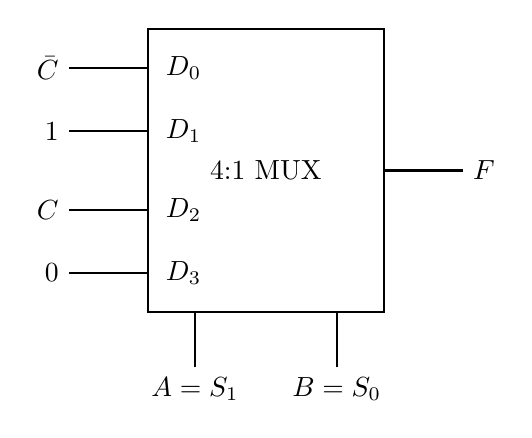
\begin{tikzpicture}[line width=.8pt]
\draw (0,0) rectangle (3,3.6);\node at (1.5,1.8) {4:1 MUX};
\foreach \y/\d/\v in {3.1/0/{\bar C},2.3/1/1,1.3/2/C,.5/3/0}{
 \draw (-1,\y) node[left] {$\v$}--(0,\y);\node[anchor=west] at (.1,\y) {$D_\d$};}
\draw (3,1.8)--(4,1.8) node[right] {$F$};
\draw (.6,-.7) node[below] {$A=S_1$}--(.6,0);
\draw (2.4,-.7) node[below] {$B=S_0$}--(2.4,0);
\end{tikzpicture}\end{center}
Generate $\bar C$ with one CMOS inverter if it is not already available.
This uses one 4:1 multiplexer, as requested, rather than an unrestricted 2:1 tree.
\begin{center}\begin{tabular}{cccc@{\qquad}cccc}\toprule
$A$&$B$&$C$&$F$&$A$&$B$&$C$&$F$\\\midrule
0&0&0&1&1&0&0&0\\0&0&1&0&1&0&1&1\\
0&1&0&1&1&1&0&0\\0&1&1&1&1&1&1&0\\\bottomrule
\end{tabular}\end{center}
All eight cases are checked independently against the printed Boolean expression.
No complete local submitted HW1 answer accompanies the prompt; the MOS proof
attachment covers Questions 1 and 2 only. The remaining designs are derived here.

\newpage\section*{4(a). Static CMOS with two nested overbars}
The outer bar covers the whole sum, and the inner bar covers $(x+y)$:
\[
 \boxed{f=\overline{w\,\overline{(x+y)}+yz}.}
\]
First generate $h=\overline{x+y}$ with a four-transistor NOR. Then use an
eight-transistor AOI22 gate: its PDN is $(n_w\text{ series }n_h)$ in parallel
with $(n_y\text{ series }n_z)$; the dual PUN is $(p_w\parallel p_h)$ in series
with $(p_y\parallel p_z)$. Only true \emph{external} inputs are required.
\begin{center}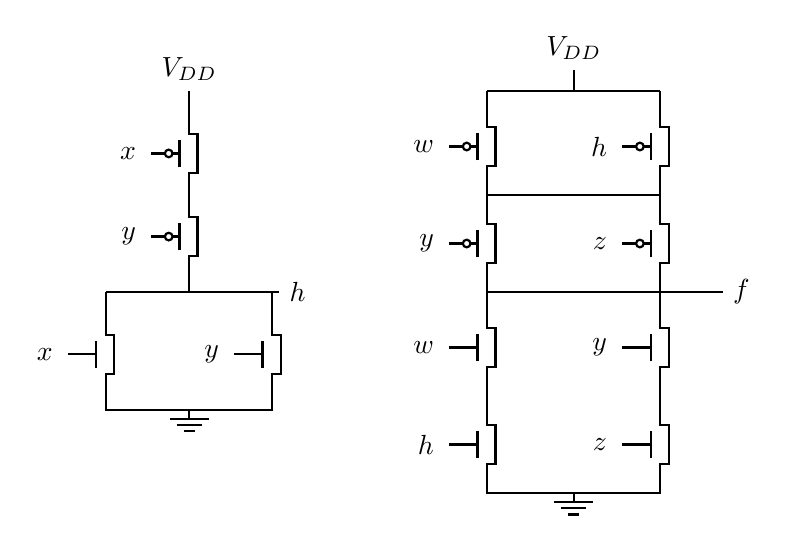
\begin{tikzpicture}[line width=.8pt,x=.88cm,y=.88cm]
\PM{HP1}{-1}{5.1}{x}\PM{HP2}{-1}{3.9}{y}
\draw (HP1t)--(-1,6) node[above] {$V_{DD}$};\draw (HP1b)--(HP2t);
\draw (HP2b)--(-1,3.1)--(.3,3.1) node[right] {$h$};
\NM{HN1}{-2.2}{2.2}{x}\NM{HN2}{.2}{2.2}{y}
\draw (-2.2,3.1)--(.2,3.1);\draw (HN1t)--(-2.2,3.1);\draw (HN2t)--(.2,3.1);
\draw (HN1b)--(-2.2,1.4)--(.2,1.4)--(HN2b);\groundat{-1}{1.4}
\PM{AP1}{3.3}{5.2}{w}\PM{AP2}{5.8}{5.2}{h}
\PM{AP3}{3.3}{3.8}{y}\PM{AP4}{5.8}{3.8}{z}
\draw (3.3,6)--(5.8,6);\draw (4.55,6)--(4.55,6.3) node[above] {$V_{DD}$};
\draw (AP1t)--(3.3,6);\draw (AP2t)--(5.8,6);
\draw (AP1b)--(3.3,4.5)--(5.8,4.5)--(AP2b);
\draw (AP3t)--(3.3,4.5);\draw (AP4t)--(5.8,4.5);
\draw (AP3b)--(3.3,3.1)--(5.8,3.1)--(AP4b);\draw (5.8,3.1)--(6.7,3.1) node[right] {$f$};
\NM{AN1}{3.3}{2.3}{w}\NM{AN2}{3.3}{.9}{h}
\NM{AN3}{5.8}{2.3}{y}\NM{AN4}{5.8}{.9}{z}
\draw (AN1t)--(3.3,3.1);\draw (AN3t)--(5.8,3.1);
\draw (AN1b)--(AN2t);\draw (AN3b)--(AN4t);
\draw (AN2b)--(3.3,.2)--(5.8,.2)--(AN4b);\groundat{4.55}{.2}
\end{tikzpicture}\end{center}
The two diagrams share the labeled $h$ signal. Total: $4+8=\boxed{12}$ MOSFETs.
The checker solves the NOR's actual switch network before evaluating the AOI22
network, then tests all 16 input words against the nested expression. Removing
the inner bar would produce a different function; it is not a permissible
reuse of a later year's AOI diagram.

\newpage\section*{4(b). Complement of three-input majority}
\[
 f=\bar x\bar y+\bar x\bar z+\bar y\bar z
 =\overline{xy+xz+yz}=\overline{x(y+z)+yz}.
\]
The PDN is $n_x$ in series with $(n_y\parallel n_z)$, in parallel with
$n_y$ in series with $n_z$. The PUN is its series/parallel dual.
\begin{center}\AOIcircuit{x}{y}{z}{y}{z}\par
\textbf{Minority gate: 5 NMOS + 5 PMOS.}\end{center}
It is high for input Hamming weight 0 or 1 and low for weight 2 or 3. No
external complemented inputs are needed: PMOS gate bubbles supply the
complementary switch-enable condition. All eight states have exactly one
conducting rail network.
\textbf{Verification.} Run \texttt{python verify.py}. All 32 Boolean/switch
cases and all 80,800 long-channel operating points pass. Results are preserved
in \texttt{truth\_tables.csv} and \texttt{verification.json}. These are ideal
logic and model-equation checks, not physical SPICE timing measurements.

\end{document}
